\section[Dense Representation]{Dense Representation: The Good, The Bad, and The Pointers}%
\label{sec:overview}
\label{ssec:overview:dense}
%\rn{Lovely section title!}

This section gives a refresher on dense representations of algebraic datatypes (\Secref{sec:overview:overview})
and, using an example, illustrates the performance challenges of picking a
layout for a datatype's dense representation (\Secref{sec:overview:example}).

\subsection{Overview}%
\label{sec:overview:overview}

\emph{Algebraic datatypes} (ADTs) are a powerful language-based technology. ADTs can
express many complex data structures while, nevertheless, providing a
pleasantly high level of abstraction for application programmers.
% ADTs are directly supported in many functional languages, such as Haskell and
% dialects of ML, and can be modeled in object-oriented languages via restricted
% forms of classes (sealed classes in Java, case classes in Scala, etc.).
The high-level specification of ADTs leaves
space to experiment with low-level implementation strategies. Hence, we use ADTs
and a purely functional setting for our exploration of performance implications of
data layout.

%\paragraph{Mostly dense data representation in \gibbon{}.}
%
In a conventional implementation of algebraic datatypes, accessing a value of a
given ADT requires dereferencing a pointer to a heap object, then reading the
header word, to get to the payload.
% Getting to the
% payload may require one more pointer dereference.
Accessing the desired data may require multiple further pointer dereferences, as objects
may contain pointers to other objects, requiring the unraveling of multiple layers of nesting.
% \Red{It may require more than one pointer dereference because of the nested degree of \textit{indirections},
% that is, a pointer could store the location of another pointer which then carries the actual data?}
% \vs{TODO: Audit this part}
%
The whole process is often described as \emph{pointer chasing}, a fitting name, 
especially when the work per payload element is low.

In a dense representation of ADTs, as implemented in \gibbon{},
the data constructor stores
one byte for the constructor's {\em tag}, followed immediately by its fields,
in the hope of avoiding pointer chasing.
%
Wherever possible, the tag value occurs inline in a bytestream that
hosts multiple values.
%
As a result, values tend to reside compactly in the heap using contiguous blocks of
memory. This representation avoids or reduces pointer chasing and admits
efficient linear traversals favored by modern hardware via
prefetching and caching.
%% %
%% In contrast, such efficiency is either impossible or extremely
%% challenging for the approaches taken by most other functional
%% languages, where there is a more conventional treatment of algebraic
%% datatypes.
%% %
%% Such approaches resort to fully or mostly boxed representations of
%% values, and often the tradeoffs are made in the compiler in ways that
%% are hard for novice or even expert application programmers to
%% anticipate.

%\paragraph{Where dense representation falls short.}

\subsection{Running Example}%
\label{sec:overview:example}

The efficiency of traversals on dense representations of data structures
largely depends on how well access patterns and layout match each other.
%
Consider a datatype (already monomorphized) describing
a sequence of posts in a blog\footnote{Throughout the paper we use a subset of Haskell syntax, which
corresponds to the input language of the \gibbon compiler.}:
\begin{lstlisting}
    data BlogList = Nil | Blog Content HashTags BlogList
\end{lstlisting}
%
A non-empty blog value stores a content field (a
string representing the body of the blog post), a list of hash tags
summarizing keywords of the blog post, and a pointer to the rest of
the list.%
%
\footnote{%
  In practice, you may want to reuse a standard list type, e.g.:
  \begin{lstlisting}
    type BlogList = [Blog]
    data Blog = Blog Content HashTags
\end{lstlisting}
 but a typical compiler (including
  \gibbon) would specialize the parametric list type with the \lstinline|Blog|
  type to arrive at an equivalent of the definition shown in the main text
  above.%
}. The datatype has one point of recursion and several variable-length fields in
the definition. To extend on this, \Secref{subsec:eval:trees:rightmost} contains
an example of tree-shaped data (two points of recursion, in particular) with a
fixed-length field. The most general case of multiple points of recursion and
variable-length fields is also handled by \system.

The most favorable traversal for the \lstinline|Blog| datatype
is the same as the order in
which the fields appear in the datatype definition. In this case, \gibbon{} can
assign the dense and pointer-free layout as shown in Figure~\ref{fig:traversal-ideal}.
Solid blue arrows connecting adjacent fields represent unconditional sequential
accesses---i.e., reading a range of bytes in a buffer, and then reading the next
consecutive range.
Such a traversal will reap the benefits of locality.

\begin{figure}[t]
  \begin{lstlisting}[]
  emphKeyword :: String -> BlogList -> BlogList
  emphKeyword keyword blogs = case blogs of
      Nil -> Nil
      Blog content hashTags blogs' ->
          case search keyword hashTags of
            True -> let content' = emphContent content keyword
                        blogs''  = emphKeyword keyword blogs'
                      in Blog content' hashTags blogs''
            False -> let blogs'' = emphKeyword keyword blogs'
                       in Blog content hashTags blogs''
   \end{lstlisting}
  \caption{Blog traversal motivating example}
  \label{fig:blog-traversal}
\end{figure}

%\begin{center} 

%\end{center}

%
% Artem: vv--this blows out the suspense!
%There is no work to compute the \emph{start} of a downstream field,
%because its starting address is at the end of the preceding field!

%\paragraph{Skipping over fields of a datatype.}
%
On the other hand, consider a traversal with less efficient access patterns (\figref{fig:blog-traversal}).
%
The algorithm scans blog entries for a given keyword in \lstinline|HashTags|.
%
If the hash tags of a particular blog entry contain the keyword, the
algorithm puts an emphasis on every occurrence of the keyword in the content
field.
%
In terms of access patterns, if we found a match in the hash tags field,
subsequent accesses to the fields happen in order, as depicted in Figure~\ref{fig:traversal-blog-time-complexity-left}.
%
Otherwise, the traversal skips over the content field, as depicted in Figure~\ref{fig:traversal-blog-time-complexity-right}.
%
% \begin{center}
%   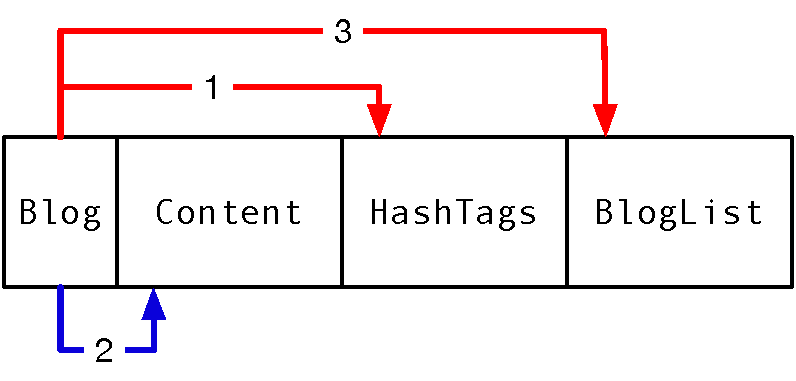
\includegraphics[width=0.4\linewidth]{figures/traveral_blog_then_gibbon_time_complexity.pdf} \, \,
%     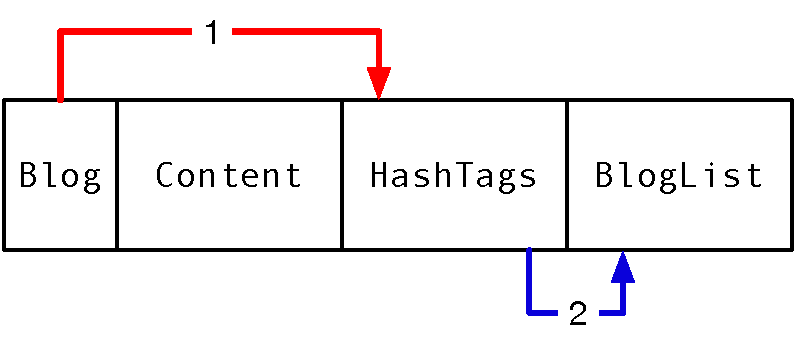
\includegraphics[width=0.4\linewidth]{figures/traveral_blog_else_gibbon_time_complexity.pdf}
% \ap{I think they should be a proper Figure}
% \end{center}

%\begin{center}

%\end{center}


%
Here we use red lines to represent accesses that must \emph{skip over} some data
between the current position in the buffer and the target data. \new{Data may be constructed recursively
and will not necessarily have a statically-known size, so finding the end of a piece of unneeded data requires
scanning through that data in order to reach the target data.}
%
This \new{extra traversal (parsing data just to find the end of it)} requires an arbitrarily large amount of work because
the \lstinline|content| field has a variable, dynamically-allocated size. 
%There is
%no way of knowing where it ends without storing a pointer to the start of \lstinline|HashTags|.

% \begin{figure}[t]
%     \begin{minipage}[c]{\linewidth}
%     \centering
%     \subfloat[][True case]{
%       \centering
%     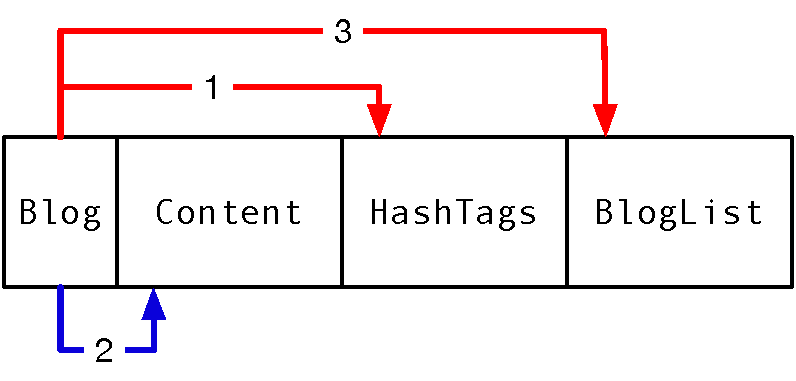
\includegraphics[width=0.4\textwidth]{figures/traveral_blog_then_gibbon_time_complexity.pdf}\label{fig:traversal-blog-time-complexity-left}}
%     \subfloat[][False case]{
%       \centering
%     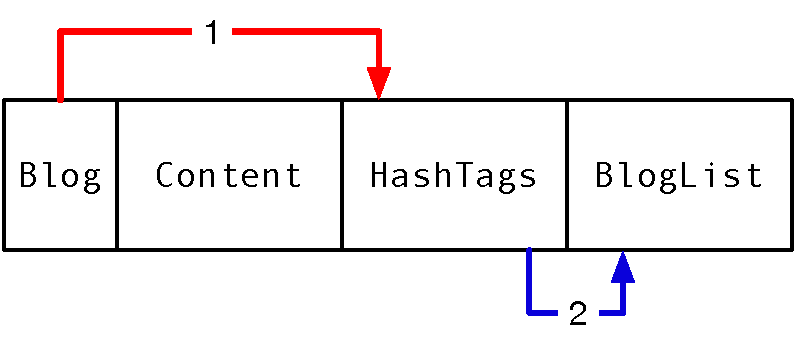
\includegraphics[width=0.4\textwidth]{figures/traveral_blog_else_gibbon_time_complexity.pdf}\label{fig:traversal-blog-time-complexity-right}}
%     \label{fig:traversal-blog-time-complexity}
%     \caption{\ap{alignment of pictures and captions looks off}\new{Out of order accesses (red), incurring costly extra traversals over fields in the middle.}}
%   \end{minipage}\hfill
% \end{figure}

%\paragraph{Shortcut pointers.}
%
\new{Extra traversals that perform useful no work}, like skipping over the \lstinline|content| field above,
can degrade the asymptotic efficiency of programs.
%
One way to avoid such traversals is to use pointers.
%
For instance, when \gibbon detects that it has to skip over intervening data, it
changes the definition of the constructor by inserting \emph{shortcut pointers},
which provide an exact memory address to skip to in constant time.
% (similar in spirit to pointer swizzling). % Artem: <- what's that??
%
For our example program, \gibbon{} introduces one shortcut
pointer for the \lstinline|HashTags| field, and another one for the tail of the list.
%

  % \begin{figure}[t]
  %   \begin{minipage}[c]{\linewidth}
  %   \centering
  %   \subfloat[][True case]{
  %   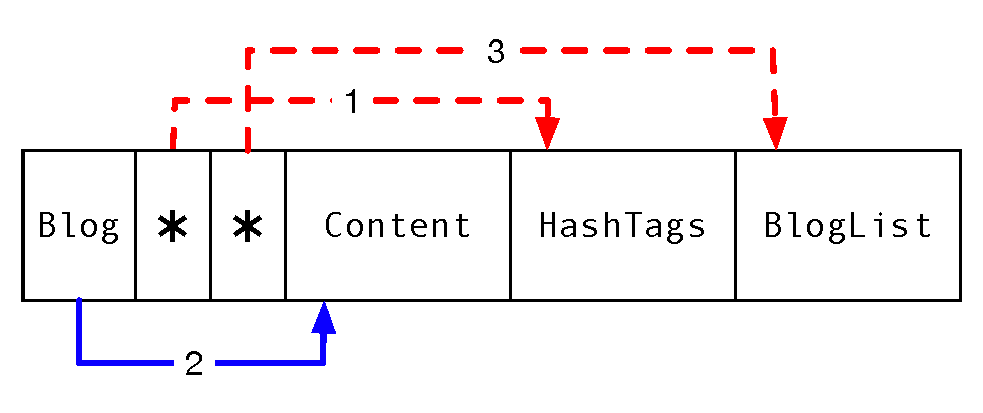
\includegraphics[width=0.4\textwidth]{figures/traveral_blog_then_gibbon_pointers.pdf}\label{fig:traversal-blog-pointers-left}}
  %   \subfloat[][False case]{
  %   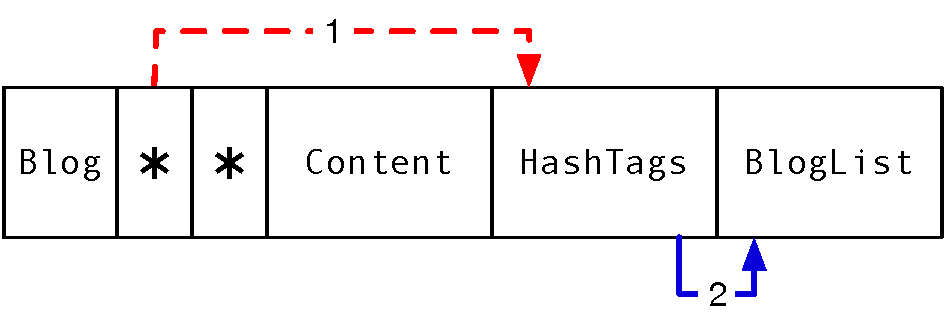
\includegraphics[width=0.4\textwidth]{figures/traveral_blog_else_gibbon_pointers.pdf}\label{fig:traversal-blog-pointers-right}}
  %   \caption{Representation with pointers to allow random access.}
  %   \label{fig:traversal-blog-pointers}
  % \end{minipage}\hfill
  % \end{figure}

The pointers provide direct accesses to the respective fields when needed and
restore the constant-time asymptotic complexity for certain operations.
\new{This results in the access patterns shown in Figure~\ref{fig:traversal-blog-pointers-left} and~\ref{fig:traversal-blog-pointers-right}.}
Red dashed lines represent pointer-based constant-time field accesses.
%
Otherwise, the access patterns are similar to what we had before.

The pointer-based approach in our example has two weaknesses. First, this
approach is susceptible to the usual problems with pointer chasing. Second, just
like with the initial solution, we access fields in an order that does not match
the layout: the hash tags field is always accessed first but lives next to the
content field. 
%In the next subsection we give an overview of our analysis, which
%helps to improve this example and results in the access patterns shown in Figure~\ref{fig:traversal-blog-optimized}.

\system, described in the following section, automates finding
the weaknesses of the pointer-based approach and improving data layout and code accordingly.
For instance, performance in our example can be improved by swapping the
ordering between the \lstinline|Content| and \lstinline|HashTags| fields.
%
Given this reordering, the hash tags are available directly at the start of the
value, which lines up with the algorithm better, as the algorithm always
accesses this field first.
%
Additionally, our program's \lstinline|True| case (the keyword gets a hit within the
hash tags) is more efficient because after traversing the content to highlight
the keyword it stops at the next blog entry ready for the algorithm to make
the recursive call.
%
This improved data layout results in the more-streamlined access patterns shown in Figures~\ref{fig:traversal-blog-optimized-left} and~\ref{fig:traversal-blog-optimized-right}.
%
%\begin{center}
%  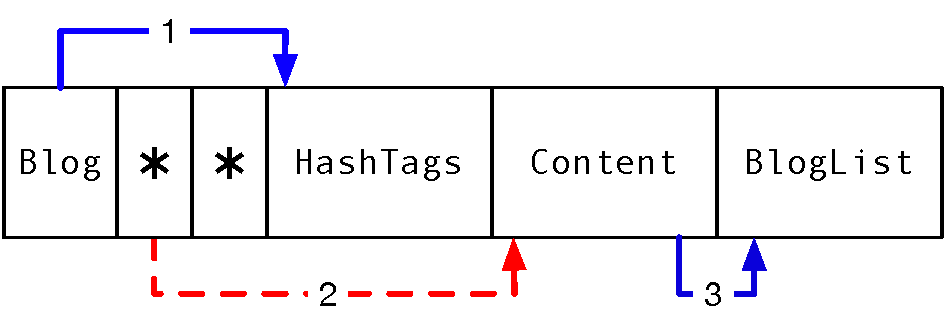
\includegraphics[width=0.4\linewidth]{figures/traveral_blog_then_gibbon_optimized.pdf} \, \,
%  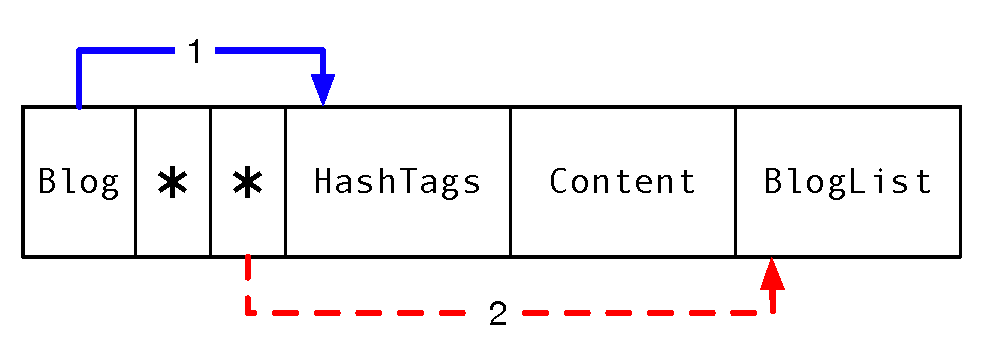
\includegraphics[width=0.4\linewidth]{figures/traveral_blog_else_gibbon_optimized.pdf}
%\end{center}
%\vspace{-2.8em}
%\begin{center}

%\caption{Optimized layout with favorable access patterns.}
%  \label{fig:traversal-blog-pointers}

\begin{figure}[t]
  \centering
  \captionsetup[subfigure]{justification=centering}
\begin{subfigure}{0.43\textwidth}
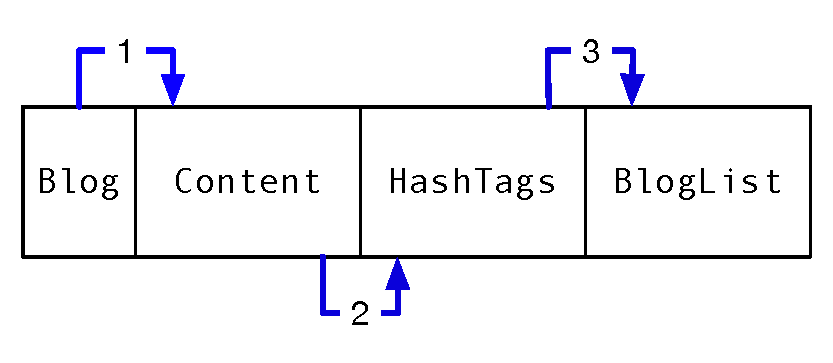
\includegraphics[width=\textwidth]{figures/Ideal_serial_layout_linear_access.pdf}
\caption{{Ideal access patterns}}
\label{fig:traversal-ideal}
\end{subfigure}
\\
\begin{subfigure}{0.43\textwidth}
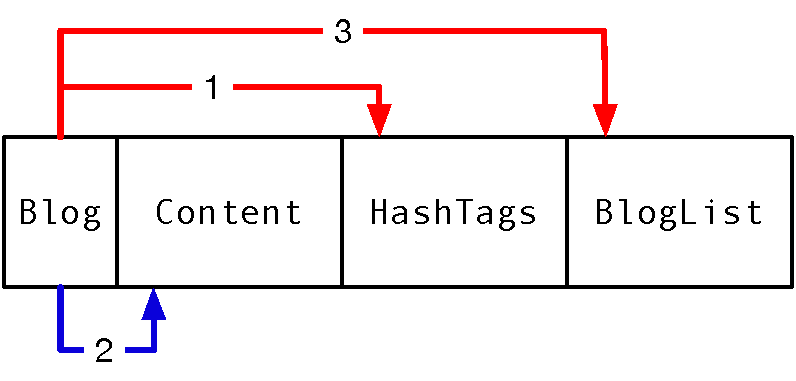
\includegraphics[width=\textwidth]{figures/traveral_blog_then_gibbon_time_complexity.pdf}
\caption{{True case extra traversals}}
\label{fig:traversal-blog-time-complexity-left}
\end{subfigure}
\begin{subfigure}{0.43\textwidth}
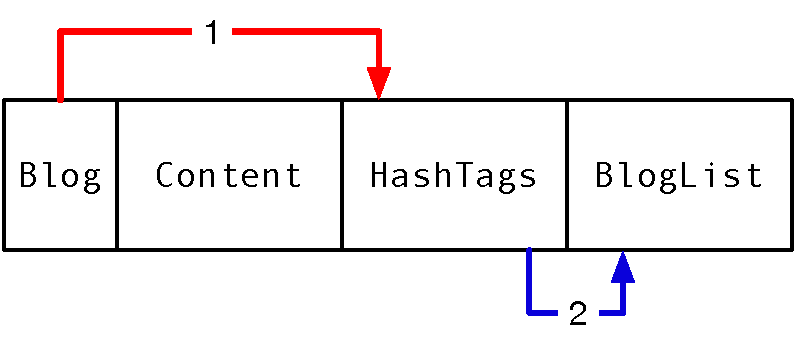
\includegraphics[width=\textwidth]{figures/traveral_blog_else_gibbon_time_complexity.pdf}
\caption{{False case extra traversals}}
\label{fig:traversal-blog-time-complexity-right}
\end{subfigure}
\caption{Showing a dense pointer-free layout with ideal accesses on top. Numbers represent the access order. 
          Out of order accesses (red), incur costly extra traversals over fields in the middle.}
\end{figure}


\begin{figure}[t]
  \captionsetup[subfigure]{justification=centering}
  \begin{minipage}[]{\linewidth}
  \centering
  \subfloat[][{True case unoptimized}]{
  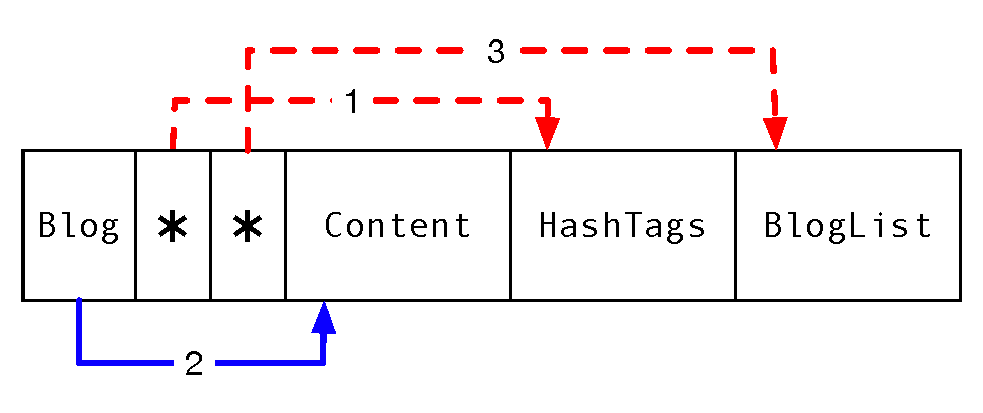
\includegraphics[width=0.50\textwidth]{figures/traveral_blog_then_gibbon_pointers.pdf}\label{fig:traversal-blog-pointers-left}}
  \subfloat[][{True case optimized}]{
  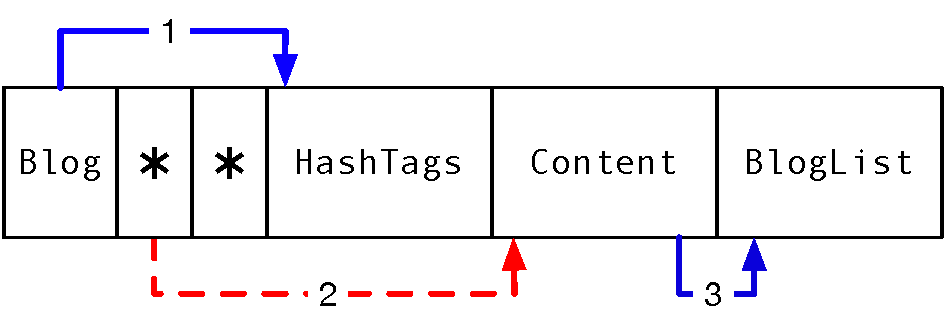
\includegraphics[width=0.50\textwidth]{figures/traveral_blog_then_gibbon_optimized.pdf}\label{fig:traversal-blog-optimized-left}}
  \\
  \subfloat[][{False case unoptimized}]{
  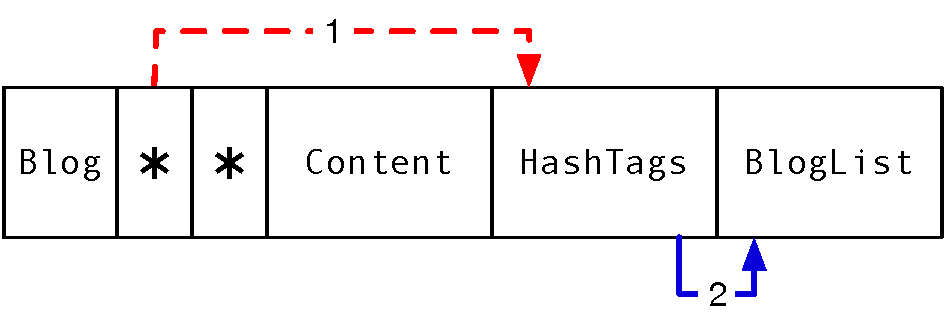
\includegraphics[width=0.50\textwidth]{figures/traveral_blog_else_gibbon_pointers.pdf}\label{fig:traversal-blog-pointers-right}}
  \subfloat[][{False case optimized}]{
  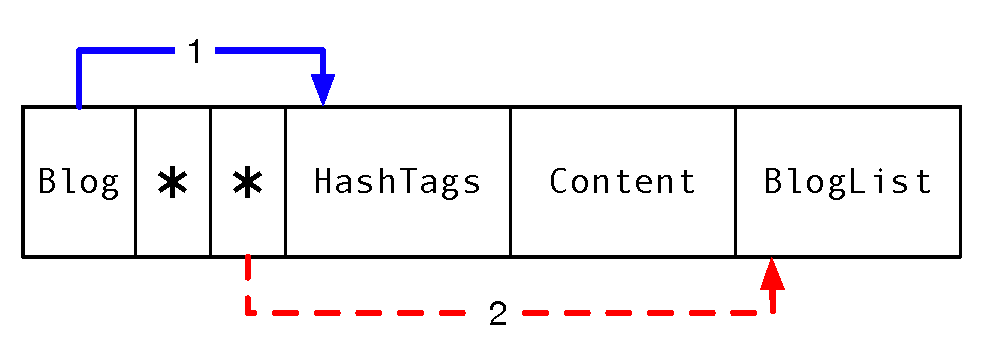
\includegraphics[width=0.50\textwidth]{figures/traveral_blog_else_gibbon_optimized.pdf}\label{fig:traversal-blog-optimized-right}}
  \caption{Showing the unoptimized representation with pointers to allow random access and the optimized layout with favorable access patterns.}
\end{minipage}\hfill
\end{figure}
%\end{center}



% %
% This improved layout is produced automatically by \system{}.

% Yet, there remains plenty of room for improvement: if we optimize the
% data layout for this specific program, we can (1) further compact our
% blog items by doing with just one shortcut pointer and (2) achieve
% a better, more linear traversal in the ``then'' branch.
% %
% To get these improvements, we design an approach that combines
% type-level and control-flow information and restructures the program
% accordingly.

% Artem: the next subsection largely repeats contributions from Intro and doesn't
% provide new insights in how the system works. In the interest of space as well
% as presentation I mute it for the time being. I think what it was supposed to
% do (show how the system works using the BlogList example) is achieved in
% section 3.
% \subsection{Picking A Better Layout With \system}
% \label{ssec:overview:marmoset}

% % Artem: vv--this all has been said and will be repeated again many times.
% %                Let's just focus on an example...
% % Our approach is to increase compactness and linear access by taking
% % into account temporal access patterns in the program.
% % %
% % Given the results of a program analysis, we reorder the fields in type
% % constructors (and adjust the code accordingly).
% %
% % Artem: [future work]
% %        let's not reiterate the point that we did not implement (below).
% % We note that, although our depictions above show two shortcut
% % pointers, our \system{} actually enables a significant compaction,
% % thanks its reordering of the fields.
% %
% % With reordering, we can remove the first shortcut pointer, that is,
% % the one pointing to the content field, because each of the two
% % conditional branches in our program already fully traverse the
% % hash-tags field, and thus already pay for finding the starting address
% % of the content field.
% %
% % However, to realize this single-pointer version, there some
% % improvements to the rest of the \gibbon{} compiler that are needed,
% % and we leave such efforts to future work.

% \paragraph{Customizable layouts.}
% %
% In \system{}, we treat data ordering as a free variable, adapting
% it to the code that uses the data.
% %
% % Artem: [future work]
% % We also provide annotations, which the user can add in comments to
% % partially or fully constrain the search space of orderings
% % (narrowing).
% %
% There are also examples where widening the search space to include
% transformations of the \emph{program order} as well would yield even
% better solutions, which could complement our approach, Infact, we use
% \textit{code-motion} of let bindings as another free variable in our
% optimization and talk about when we use it to further optimize the
% running example in~\ref{sec:attributes}. If data-flow dependencies allow
% code-motion of let bindings, we place fields in such a way that mimics
% a \textit{structure of arrays} type transformation.
% Consider for example a list datatype:
% \begin{lstlisting}
% data List =  Nil | Cons Int List
% \end{lstlisting}
% Here, \lstinline|List| on the right-hand side of the equals sign is a recursive
% field representing the tail of a linked list. We show that having the element field
% (\lstinline|Int| in the example) after the tail of the list may offer similar benefits to a
% \textit{structure-of-arrays} representation if datatypes are packed by the
% compiler. This is a cherry on top of optimizing for the access patterns as discussed before.
% % Artem: the next sentence goes into too much details.
% % Since, the Integer fields are all next to each other in memory, albeit, in the reverse order.

% \paragraph{From access patterns in the program to the field-access graph, a cost model of field orderings.}
% %
% The key to our approach is a cost model that assigns costs to
% different field orderings and a compiler pass that infers costs for
% given programs and assigns fields accordingly.
% %
% Our cost model involves the inference for each data-type constructor
% in the program of a \emph{field-access graph}.
% %
% This graph represents the temporal ordering of accesses among fields
% and the associated costs, based on the control-flow and data -flow graph
% of the program.
% %
% Regarding the \lstinline|Blog| constructor, for example, our analysis produces a
% field-access graph with three vertices representing the three fields, where each
% edge means that one field is accessed immediately before the other.
% %
% The edges are induced by the two branches in our example function: in
% the ``then'' branch, we have an edge going from the hash-tags to the
% content field, and one from the content to the tail-pointer field; in
% the ``else'' branch there is an edge from the hash-tags to the
% list-tail field. Edges are differented by whether they arise from a data flow
% dependency or purely an outcome of the control flow of the program.
% Section~\ref{design:fieldgraph} talks about this distinction further.

% \paragraph{From field-access graph to optimized ordering, via ILP solver.}
% %
% From this graph, we obtain a cost model for different orderings by
% weighting each edge.
% %
% Such weights are determined in our approach by approximate properties
% of the program's control flow, e.g., the likelihood of a given access
% based on the branching structure leading to the access.
% %
% Our approach takes a simple but effective approximation based on
% static control flow and data flow, but more sophisticated approximations are
% possible.
% %
% Given a cost graph, \system{} then encodes it as an optimization problem that
% can be solved by an off-the-shelf ILP (integer linear programming) solver.
% %
% This optimization problem is tractable because its size is in
% proportion to the size of the data-type definition, not that of the
% whole program.
% %
% From the resulting ILP solution, we can decode the result and obtain
% an efficient reordering of the fields.
% %
% In general, our \system{}
% analyses one pair of function definition and data-type constructor at a time,
% and rewrites the program to reflect the reordering of its fields.
